\documentclass[utf8]{article}

\usepackage[utf8]{inputenc}

\usepackage[parfill]{parskip}

\usepackage{amsmath}
\usepackage{amssymb}
\usepackage{amsfonts}
\usepackage{graphicx}
\usepackage{float}
\usepackage{listingsutf8}
\usepackage{hyperref}
\usepackage[dvipsnames]{xcolor}

\usepackage{fullpage}

% -----------------------------------------------------


\title{Rapport}
\author{Bourgeois Noé}
\date{26 avril 2021}

\begin{document}
\maketitle
\tableofcontents

\newpage

% -----------------------------------------------------

\section{Introduction}

Le Jeu des Amazones se joue entre 2 joueurs possédant chacun 4 reines sur un plateau de 10x10 cases.
Un joueur doit lors de son tour, déplacer une de ses reines puis lui faire tirer une flèche.
Déplacement et tir se font jusqu'à une case libre dans les directions cardinales et inter-cardinales d'autant de cases libres que désirées.
Le gagnant est le joueur qui a pu jouer son tour en dernier.

Le projet d’année consistait en l'implémentation d'un programme permettant à 2 humains ou 2 IA ou 1 humain et une IA d'y jouer.

Le présent document présente une analyse approfondie et des graphiques comparatifs des différentes IA implémentées sous formes de méthodes de la classe IAPlayer,
mettant également en évidence l’influence des différents paramètres et motivant nos choix d’implémentation.


\section{Méthodes}
Dans les méthodes ci-dessous:
 L'IA, lors de son tour, simule une de ses actions possibles.
 Le paramètre de profondeur ("depth") indique le nombre de tours à simuler.
 Tant que depth est supérieur à 0, il est décrémenté de 1 et le joueur dont l'action est simulée change. l'IA simule ensuite une des actions possibles de l'adversaire puis une des siennes et recommence jusqu'à ce qu'une action mène à une victoire ou une défaite ou que depth soit à 0.
 Elle attribue alors un score à l'action puis recommence récursivement pour toutes les actions possibles de chaque tour.
 Elle finit par jouer l'action dont le score est le plus élevé.

\subsection{Minimax}
Le paramètre "maximasing", fixé par défaut à True indique qu'elle maximise le score, si une action mène à la victoire("WIN"), le score est plus élevé que si elle ne mène ni à une victoire ni à une défaite("DRAW"), plus encore que si elle mène à une défaite.


\begin{figure}[H]
\begin{minipage}{\textwidth}
  \centering
	\begin{lstlisting}
	function minimax(node, depth, maximizingPlayer) is
    if depth = 0 or node is a terminal node then
        return the heuristic value of node
    if maximizingPlayer then
        value := - INF
        for each child of node do
            value := max(value, minimax(child, depth - 1, FALSE))
        return value
    else (* minimizing player *)
        value := + INF
        for each child of node do
            value := min(value, minimax(child, depth - 1, TRUE))
        return value

(* Initial call *)
minimax(origin, depth, TRUE)
    \end{lstlisting}
  \label{fig:code_exemple}
\end{minipage}
\end{figure}

Le code de la fonction du projet est très similaire au pseudocode.
\href{https://en.wikipedia.org/wiki/Minimax}{\textcolor{blue}{Plus d'informations sur cet algorithme}} peuvent être trouvée dans de nombreuses sources de référence.

% -----------------------------------------------------
\newpage

\subsection{TournoiAIPlayer}
Le projet d'année se termine par un tournoi qui voit s'affronter les meilleures IA des étudiants. Une limite de temps a été fixée à 2 seconde après lesquelles une IA est éliminée si elle n'a pas joué une action.

\subsubsection{approfondissement itératif}
L'IA recherche donc le meilleur coup avec une profondeur de 1 puis, tant que le temps imparti n'est pas écoulé, incrémente la profondeur et recommence.

\subsubsection{m}
Dans la fonction "m" pour "aim", nous avons utilisé

\paragraph{Principal Variation Search/Negascout}:


    "\href{https://en.wikipedia.org/wiki/Principal_variation_search}{\textcolor{blue}{La recherche de variation principale}} (parfois assimilée au NegaScout pratiquement identique ) est un algorithme negamax qui peut être plus rapide que l' élagage alpha-bêta . Comme l'élagage alpha-bêta, NegaScout est un algorithme de recherche directionnelle pour calculer la valeur minimax d'un nœud dans un arbre . Il domine l'élagage alpha-bêta dans le sens où il n'examinera jamais un nœud qui peut être élagué par alpha-bêta; cependant, il repose sur un ordre précis des nœuds pour tirer parti de cet avantage.

    NegaScout fonctionne mieux quand il y a une bonne commande de coups. En pratique, l'ordre des mouvements est souvent déterminé par des recherches antérieures moins profondes. Il produit plus de seuils que l'alpha-bêta en supposant que le premier nœud exploré est le meilleur. En d'autres termes, cela suppose que le premier nœud est dans la variante principale. Ensuite, il peut vérifier si cela est vrai en recherchant les nœuds restants avec une fenêtre nulle (également appelée fenêtre de reconnaissance; lorsque alpha et bêta sont égaux), ce qui est plus rapide que la recherche avec la fenêtre alpha-bêta normale. Si la preuve échoue, alors le premier nœud n'était pas dans la variante principale et la recherche se poursuit comme une alpha-bêta normale. Par conséquent, NegaScout fonctionne mieux lorsque l'ordre des mouvements est bon. Avec un ordre de déplacement aléatoire, NegaScout prendra plus de temps que l'alpha-beta classique; bien qu'il n'explore aucun nœud  qu'alpha-beta n'a pas fait, il devra re-rechercher de nombreux nœuds."

\paragraph{Tri des actions possibles:}
    Pour optimiser la recherche de negascout la liste des actions est triée dans la fonction "aim":
    les destinations de mouvement et flèche adjacentes à une reine ennemie sont placées en début de liste.

\paragraph{Dictionnaire plateau/actions possibles:}
     Lors des simulations, chaque plateau rencontré et les actions possibles sont enregistrées dans un dictionnaire afin de ne plus devoir recommencer la recherche à la prochaine rencontre.

\paragraph{Régions et Tri des reines:}
     Une (ou plusieurs) case isolée du reste du plateau par des flèches forme une région.
    Une région d'un nombre de cases n est défective si une reine ne peut pas y effectuer n actions.
    Si une région forme une ligne, un rectangle ou un triangle, (:formes simples) et contient une seule reine, la detection de région non détective dont l'implémentation était demandée pour la partie 3 permet de déterminer son score. La fin de partie peut donc être anticipée.
    Mais les régions non défectives sont rarement de forme simple, nous avons donc implémenté à la place, un ensemble de fonctions calculant le score d'une région, défective ou non, contenant une ou plusieurs reines.
    Nous ne l'avons pas réutilisée pour TournoiAIPlayer car ce temps de calcul est potentiellement non raisonnable.
    Si une reine es isolée, une action de sa part ne fera, au mieux, que réduire la taille de sa région et donc son score de 1, au pire, elle pourrait placer sa fleche dans un goulet d'étranglement et diviser sa région en plusieurs sous régions dont les nouveaux scores sont plus petits d'au moins plus de 1. Elle est donc placée en queue de liste des reines du joueur afin qu'elle n'agisse qu'en dernier recourt.

\begin{figure}[H]
\begin{minipage}{\textwidth}
  \centering
	\lstinputlisting{./code/m.py}
  \label{fig:m}
\end{minipage}
\end{figure}

\section{Résultats}
\begin{center}
\begin{tabular}{|c|c|c|c|
                |c|c|c|c|}
\hline
plateau taille & quantité reines/joueur & timer(s) & [TournoiAIPlayer - Minimax] /20 games & M vs T \\
\hline
6              & 1                    & 1              & 14 - 6                & 13 - 7 \\
10             & 2                    & 2              & 15 - 5                & 10 - 10    \\
10             & 2                    & 1              & 16 - 4                & 6 - 14    \\
10             & 4                    & 1              & 16 - 4                & 4 - 16    \\
\hline
10             & 4                    & 2              & 13 - 7                & 13 - 7    \\
\hline
\end{tabular}
\end{center}



\begin{figure}[H]
  \centering
	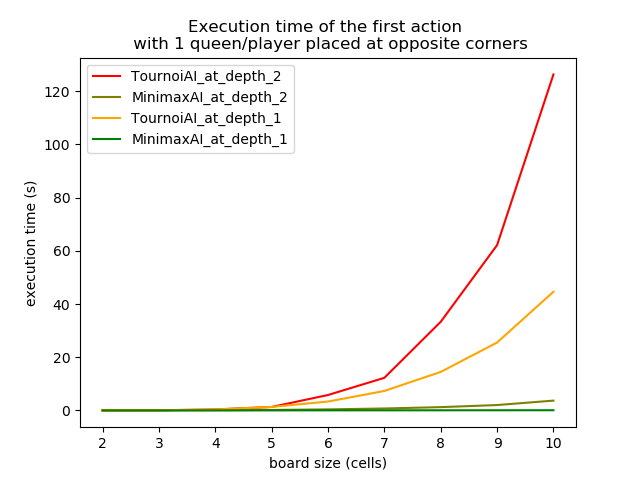
\includegraphics[scale=0.8]{img/Figure_1.png}
  \label{fig:logo}
\end{figure}

\newpage

\section{Discussion}
    Les scores de victoire sont plus serré qu'attendu.
    Nous avons donc compilé le temps d'exécution de la première action de chaque IA avec des profondeur de 1 à 2 sur des plateaux de taille 2 à 10 avec une reine par joueur chacune sur une case de coin opposé:

    Les perfomances de TournoiAIPlayer s'avèrent très mauvaises.
    Cela est dû à l'ordre des actions transmies par "aim" à Negascout. Cet ordre est bon mais manque de paramètres.

    Negascout censé être plus rapide que Minimax n'est ,ici, pas optimisé et avec une profondeur de 2, le temps d'execution double à chaque incrément de 1 de la taille de plateau.
    L'ordre des actions doit donc être mieux triée en amont..

    Une autre cause probable est que la seule heuristique (estimation de la qualité d’un scénario possible) utilisée par TournoiAIPlayer compare les scores qui restent égaux à 0 tant qu'une région n'a pas été formée.


\section{Conclusion}
Pour conclure, les idées implémentées dans TournoiAIPlayer sont intéressantes mais une mauvaise application de la principale variation search en fait une IA beaucoup plus lente que Minimax.

Elle est malgré tout victorieuse dans une majorité de parties testées dans les conditions de Tournoi grâce au tri des actions et des reines efficace peu importe la profondeur.

L'ajout (après la remise) d'heuristiques telles que le nombre d'actions possibles de l'adversaire ont considérablement amélioré les résultats.

Une optimisation du calcul de score de région via l'identification de forme simple et d'autres facteurs (que nous n'avons pas eu le temps d'implémenter mais que nous présenterons volontier dans un rapport plus long lorsque nous aurons terminé) simplifiant ce calcul l'accélèrerait significativement.

A terme, le score de région optimisé pourrait déclarer le gagnant de certaines parties avant même que celles-ci n'aient commencé.
Une IA calculant ce score serait rapide et imbattable.

\end{document}
